%  NetMasquerade — доклад (NDSS 2026), вёрстка в Beamer
\documentclass[aspectratio=169,10pt,t]{beamer}

\usepackage[english]{babel}
\babelprovide[import,main]{russian}
\usetheme{NetMasq}

\graphicspath{{figs/}}

\title{NetMasquerade}
\author{Zixuan Liu, Yi Zhao, Zhuotao Liu, Qi Li, Chuanpu Fu, Guangmeng Zhou, Ke Xu}
\date{2026}

\begin{document}

% 1. Титул
{\begin{darkslide}
\begin{frame}[plain]
\begin{tikzpicture}[remember picture,overlay]
  % декоративные точки
  \foreach \x/\c in {0/steel,1/accent,2/steel,3/accent}
    \fill[\c] ($(current page.north east)+(-3.85cm+\x*1.05cm,-1.1cm)$) circle (0.22cm);
  \foreach \x/\c in {0/steel,1/accent,2/steel}
    \fill[\c] ($(current page.north east)+(-3.85cm+\x*1.05cm,-2.15cm)$) circle (0.22cm);
  \node[anchor=north west,text width=13.2cm,align=left,inner sep=0pt] at ($(current page.north west)+(0.95cm,-1.25cm)$) {%
    {\scriptsize\bfseries\color{accentlt}NDSS Symposium 2026}\par\vspace{5mm}
    {\headfont\bfseries\fontsize{27}{30}\selectfont\color{white}NetMasquerade}\par\vspace{5mm}
    {\normalsize\color{white!92!navy}Атака уклонения по «жёсткой метке» в режиме чёрного ящика на ML-системы обнаружения вредоносного трафика}\par\vspace{5mm}
    \ico[0.75cm]{accent}{ic_mask_w.png}\hspace{2.5mm}{\scriptsize\itshape\color{white}Маскировка вредоносного трафика под легитимный с помощью Traffic-BERT + Reinforcement Learning}\par
    \vspace{5mm}{\color{steel}\rule{13.2cm}{0.5pt}}\par\vspace{4mm}
    {\scriptsize\bfseries\color{white}Zixuan Liu, Yi Zhao, Zhuotao Liu, Qi Li, Chuanpu Fu, Guangmeng Zhou, Ke Xu}\par\vspace{0.6mm}
    {\tiny\color{cardline}Tsinghua University · Beijing Institute of Technology · Zhongguancun Lab}\par\vspace{3.5mm}
    {\scriptsize\itshape\color{cardline}Докладчики: Пашков В.\,С., Штребель А.\,А., Реймер С.\,В. \ · \ группа ПИ-12 \ · \ 2026}
  };
\end{tikzpicture}
\end{frame}
\end{darkslide}}

% 2. План
\newcommand{\plancard}[4]{%
  \begin{wcard}[height=1.6cm,valign=center]
    \begin{tikzpicture}[overlay]
      \node[anchor=north east,inner sep=0pt] at (\linewidth,0.35cm)
        {\headfont\bfseries\Large\color{cardline}#1};
    \end{tikzpicture}%
    \iconitem{navy}{#2}{{\bfseries\small\color{navy}#3}\par\vspace{0.5mm}\desc{#4}}
  \end{wcard}}
\begin{frame}{План доклада}
\vspace{2mm}
\begin{columns}[T,onlytextwidth]
\column{0.485\textwidth}
  \plancard{01}{ic_crosshairs_w.png}{Контекст и проблема}{ML-детекторы трафика и их уязвимость}\par\vspace{4.5mm}
  \plancard{03}{ic_brain_w.png}{Ключевая идея}{От «жёсткой метки» к обучению с подкреплением}\par\vspace{4.5mm}
  \plancard{05}{ic_chart_w.png}{Эксперименты}{6 детекторов, 80 сценариев, метрики}
\column{0.485\textwidth}
  \plancard{02}{ic_shield_w.png}{Модель угроз}{Что известно и не известно атакующему}\par\vspace{4.5mm}
  \plancard{04}{ic_layers_w.png}{Архитектура}{Traffic-BERT + RL: две стадии}\par\vspace{4.5mm}
  \plancard{06}{ic_balance_w.png}{Защиты и выводы}{Устойчивость, ограничения, значение}
\end{columns}
\end{frame}

% 3. ML-обнаружение
\begin{frame}{ML-обнаружение вредоносного трафика}
\framesubtitle{Новая парадигма сетевой безопасности}
\vspace{1mm}
\begin{columns}[T,onlytextwidth]
\column{0.44\textwidth}
\begin{card}[height=5.9cm]
  \cardtitle{Почему ML вытесняет правила}\vspace{1mm}
  \iconitem{steel}{ic_eye_w.png}{Работает с зашифрованным трафиком — не смотрит в payload, только статистика}\vspace{4mm}
  \iconitem{steel}{ic_bolt_w.png}{Ловит неизвестные и сложные атаки лучше сигнатурных методов}\vspace{4mm}
  \iconitem{steel}{ic_server_w.png}{Развёртывается на «железе»: программируемые коммутаторы, SmartNIC}
\end{card}
\column{0.53\textwidth}
\begin{wcard}[height=5.9cm]
  \cardtitle{Признаки, на которых учатся детекторы}
  \centering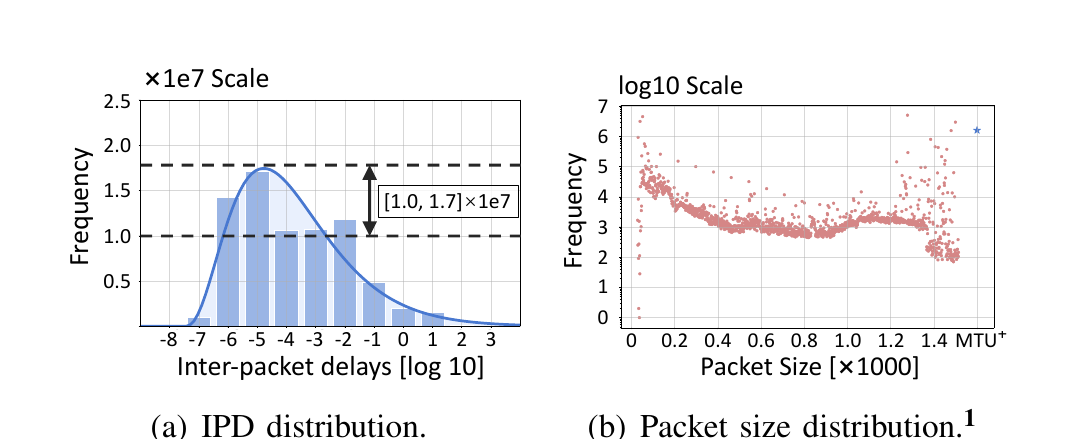
\includegraphics[width=0.94\linewidth]{fig4.png}\par\vspace{1.2mm}
  \raggedright\figcap{Размеры пакетов и межпакетные задержки (IPD) — базовые статистики потока}\par\vspace{2mm}
  \begin{darkcard}[top=1.8mm,bottom=1.8mm]\scriptsize
    Примеры детекторов: Whisper, FlowLens, NetBeacon, Kitsune, \mbox{CICFlowMeter+MLP}
  \end{darkcard}
\end{wcard}
\end{columns}
\end{frame}

% 4. Проблема
\newcommand{\limcard}[3]{%
  \begin{wcard}[height=2.75cm]
    \iconitem{steel}{#1}{\bfseries\color{navy}#2}\par\vspace{3mm}
    \desc{#3}
  \end{wcard}}
\begin{frame}{Проблема: устойчивость ML почти не изучена}
\framesubtitle{Атакующий может подделать трафик и обойти детектор}
\vspace{1mm}
\begin{card}
  \iconitem{badred}{ic_bug_w.png}{\hl{Adversarial-трафик:} добавляя, задерживая или изменяя пакеты, атакующий заставляет модель классифицировать вредоносный поток как легитимный.}
\end{card}\par\vspace{4mm}
{\small\bfseries\color{navy}Ограничения существующих атак}\par\vspace{2.5mm}
\begin{columns}[T,onlytextwidth]
\column{0.315\textwidth}\limcard{ic_lock_w.png}{Узкие условия}{Требуют Tor, туннелей, шифрования или спец-настроек — ломаются при смене среды}
\column{0.315\textwidth}\limcard{ic_eye_w.png}{Много знаний о цели}{White-box (градиенты) / gray-box (данные, признаки) — нереалистично}
\column{0.315\textwidth}\limcard{ic_arrows_w.png}{Не переносятся}{Заточены под один протокол/задачу, плохо работают в разнородной среде}
\end{columns}
\end{frame}

% 5. Открытый вопрос
\newcommand{\qcard}[3]{%
  \begin{navycard}[height=1.25cm,valign=center]
    \iconitem{accent}{#1}{{\bfseries\color{white}#2}\par\vspace{0.4mm}{\scriptsize\color{cardline}#3}}
  \end{navycard}}
{\begin{darkslide}
\begin{frame}
\vspace{12mm}
{\scriptsize\bfseries\color{accentlt}Открытый вопрос}\par\vspace{3mm}
{\headfont\bfseries\fontsize{17}{21}\selectfont\color{white}Возможна ли атака уклонения по\\«жёсткой метке» в чистом чёрном ящике?}\par\vspace{7mm}
\begin{columns}[T,onlytextwidth]
\column{0.485\textwidth}
  \vspace{2mm}\qcard{ic_random_w.png}{Протокол-агностична}{любой трафик: шифрованный, туннель, обычный}\par\vspace{5mm}
  \qcard{ic_eye_w.png}{Только «прошёл / не прошёл»}{единственный сигнал — блокирует ли система пакеты}
\column{0.485\textwidth}
  \vspace{2mm}\qcard{ic_puzzle_w.png}{Задаче-агностична}{сканирование, DoS, ботнеты, веб-атаки}\par\vspace{5mm}
  \qcard{ic_check_w.png}{Сохранение вредоносности}{минимальные правки, атака продолжает работать}
\end{columns}
\end{frame}
\end{darkslide}}

% 6. Место среди атак
\begin{frame}{Место NetMasquerade среди атак}
\framesubtitle{Единственный метод, закрывающий все требования сразу}
\vspace{2mm}
\begin{wcard}[left=1.5mm,right=1.5mm]
  \centering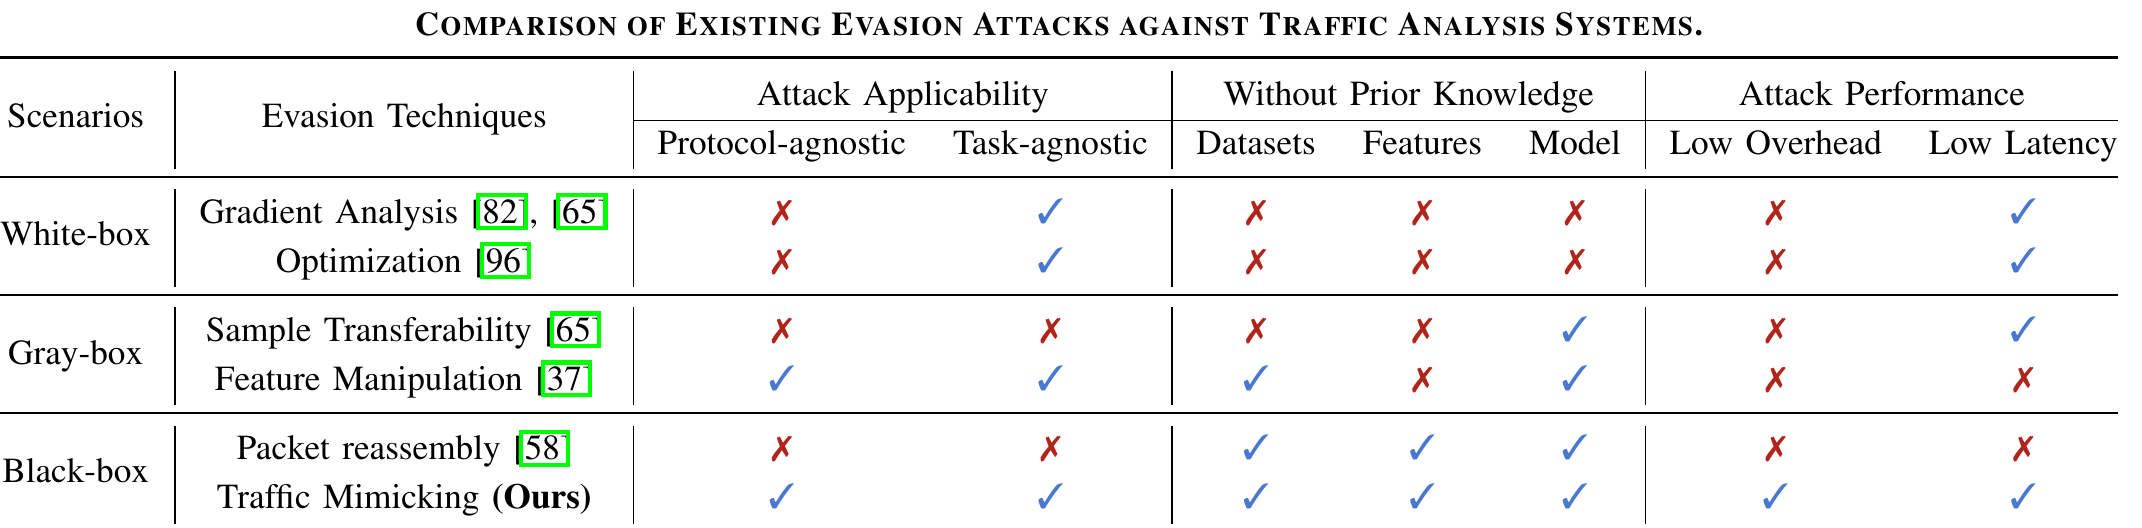
\includegraphics[width=\linewidth]{table1.png}
\end{wcard}\par\vspace{5mm}
\begin{card}
  \iconitem{accent}{ic_flag_w.png}{\hl{Ours (Traffic Mimicking):} протокол- и задаче-агностична, не требует данных / признаков / модели цели, при этом низкие накладные расходы и низкая задержка.}
\end{card}
\end{frame}

% 7. Модель угроз
\begin{frame}{Модель угроз}
\framesubtitle{Атакующий управляет ботнетом, детектор стоит на входе жертвы}
\vspace{1mm}
\begin{columns}[T,onlytextwidth]
\column{0.61\textwidth}
  \vspace{4mm}
  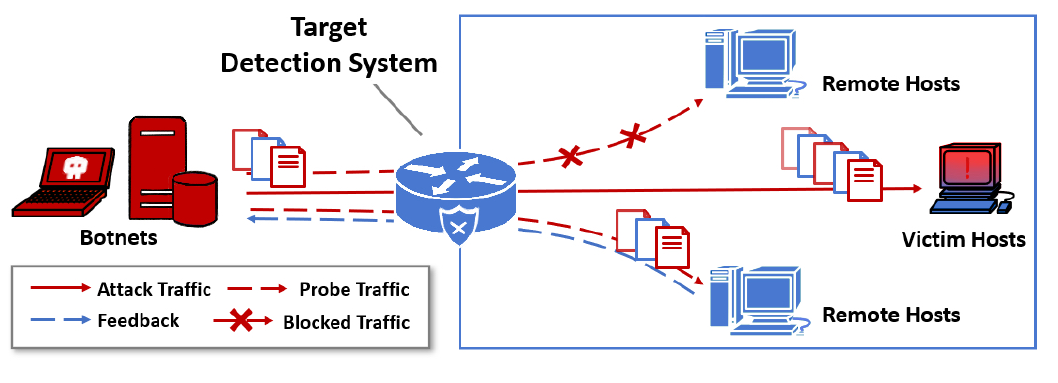
\includegraphics[width=\linewidth]{fig1.png}\par\vspace{3mm}
  \figcap{Детектор пропускает легитимный трафик и блокирует / ограничивает вредоносный.}
\column{0.36\textwidth}
\begin{darkcard}[height=5.8cm]
  \cardtitlew{Что делает система}\vspace{1.5mm}
  \iconitem[0.5cm]{navy2}{ic_check_a.png}{Работает по статистике потока (размеры, задержки), payload не смотрит}\vspace{4mm}
  \iconitem[0.5cm]{navy2}{ic_check_a.png}{Приоритет — доступность сети: дешевле дропнуть пакет, чем блокировать IP}\vspace{4mm}
  \iconitem[0.5cm]{navy2}{ic_check_a.png}{Дроп/rate-limit создаёт наблюдаемую асимметрию поведения}
\end{darkcard}
\end{columns}
\end{frame}

% 8. Разведка
\newcommand{\signalbox}[2]{%
  \begin{tcolorbox}[nmbase,colback=#1,colframe=#1,halign=flush center,valign=center,height=1.05cm,
    fontupper=\headfont\bfseries\small\color{white}]#2\end{tcolorbox}}
\begin{frame}{Разведка: как получить «жёсткую метку»}
\framesubtitle{Атакующий сам зондирует границу решения детектора}
\vspace{1mm}
\begin{columns}[T,onlytextwidth]
\column{0.49\textwidth}
\begin{card}[height=5.7cm]
  \cardtitle{Пробный трафик}\vspace{1mm}
  \iconitem{steel}{ic_arrows_w.png}{Повторяет размеры пакетов и IPD вредоносного потока, но без реального payload}\vspace{4.5mm}
  \iconitem{steel}{ic_check_w.png}{TCP: ответ (RST/ACK/SYN-ACK) = прошёл; тишина = заблокирован}\vspace{4.5mm}
  \iconitem{steel}{ic_search_w.png}{UDP/QUIC, ICMP-Unreachable, а также side-channel (TTL, IPID)}
\end{card}
\column{0.48\textwidth}
\begin{darkcard}[height=5.7cm]
  \cardtitlew{Бинарный сигнал}\vspace{1mm}
  \signalbox{okgreen}{ПРОШЁЛ \ $\rightarrow$ \ ответ получен}\par\vspace{3mm}
  \signalbox{badred}{ЗАБЛОКИРОВАН \ $\rightarrow$ \ тишина}\par\vspace{4mm}
  {\scriptsize\color{cardline}Этого сигнала достаточно, чтобы обучать RL-политику — без доступа к модели цели.}
\end{darkcard}
\end{columns}
\end{frame}

% 9. Ключевое наблюдение
\begin{frame}{Ключевое наблюдение}
\framesubtitle{Плотность распределений подсказывает направление атаки}
\vspace{1mm}
\begin{columns}[T,onlytextwidth]
\column{0.485\textwidth}
\begin{card}[height=3.1cm]
  \iconitem{steel}{ic_network_w.png}{\bfseries\small\color{navy}Легитимный трафик — плотный}\par\vspace{3mm}
  \desc{Распределения benign-потоков заполнены и разнообразны — есть куда «спрятаться».}
\end{card}
\column{0.485\textwidth}
\begin{card}[height=3.1cm]
  \iconitem{badred}{ic_bug_w.png}{\bfseries\small\color{navy}Вредоносный — разреженный}\par\vspace{3mm}
  \desc{Атака-поток лежит в редкой области. Достаточно сдвинуть его к «многообразию» benign.}
\end{card}
\end{columns}
\vspace{8mm}
\begin{darkcard}[top=3.5mm,bottom=3.5mm]
  \iconitem{accent}{ic_brain_w.png}{{\bfseries\color{accentlt}Идея:} обучаемо «сморфить» вредоносный поток в сторону benign-многообразия, сохранив семантику атаки. Границу решения ищем интерактивно — обучением с подкреплением (RL).}
\end{darkcard}
\end{frame}

% 10. Архитектура
\begin{frame}{Общая архитектура: две стадии}
\vspace{1mm}
\centering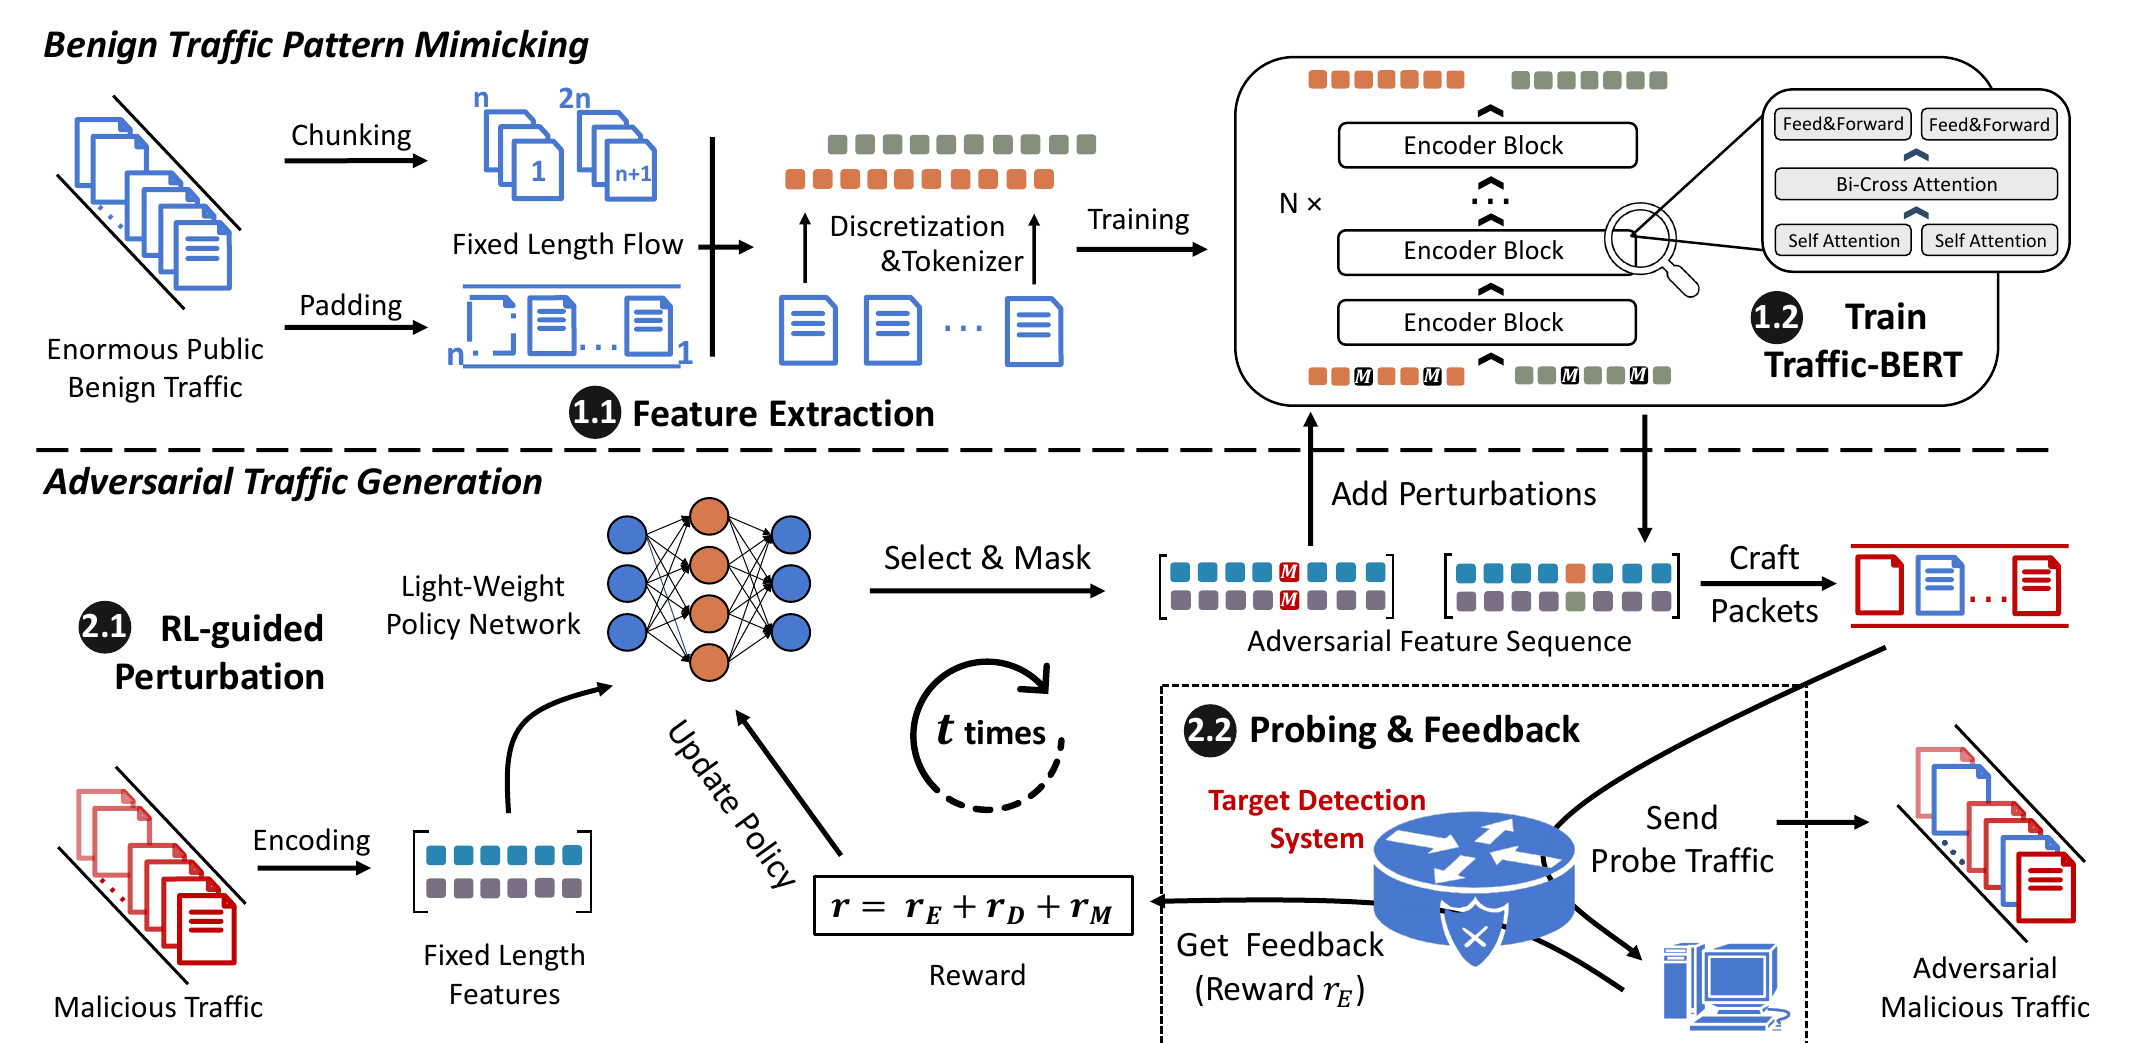
\includegraphics[height=4.85cm]{fig2.png}\par\vspace{2.5mm}
\begin{columns}[T,onlytextwidth]
\column{0.485\textwidth}
\begin{card}[top=1.6mm,bottom=1.6mm]\scriptsize
  {\bfseries\color{navy}Стадия 1} · Traffic-BERT учит паттерны легитимного трафика (офлайн).
\end{card}
\column{0.485\textwidth}
\begin{card}[top=1.6mm,bottom=1.6mm]\scriptsize
  {\bfseries\color{accent}Стадия 2} · RL-политика выбирает, где и как править пакеты (онлайн).
\end{card}
\end{columns}
\end{frame}

% 11. Стадия 1a
\begin{frame}{Стадия 1a · Извлечение признаков}
\framesubtitle{Приведение потоков к фиксированной длине и дискретным токенам}
\vspace{1mm}
\begin{columns}[T,onlytextwidth]
\column{0.49\textwidth}
  \vspace{3mm}
  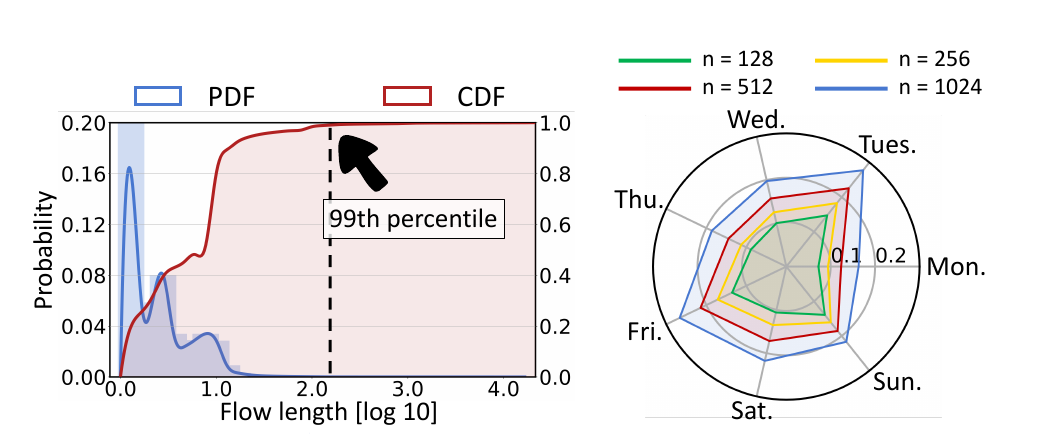
\includegraphics[width=\linewidth]{fig3.png}\par\vspace{3mm}
  \figcap{Длины потоков — «тяжёлый хвост»: берём 99-й перцентиль $\rightarrow$ $n = 512$}
\column{0.48\textwidth}
\begin{card}[height=5.8cm]\scriptsize
  \iconitem{steel}{ic_random_w.png}{\hl{Padding коротких}\ \ $m \le n$: добиваем спец-токенами [PAD]}\vspace{3.5mm}
  \iconitem{steel}{ic_layers_w.png}{\hl{Chunking длинных}\ \ $m > n$: режем на перекрывающиеся сегменты}\vspace{3.5mm}
  \iconitem{steel}{ic_code_w.png}{\hl{Токенизация}\ \ IPD $\rightarrow$ лог-интервалы; размер пакета $\rightarrow$ значение (лимит MTU, [UNK])}\vspace{3.5mm}
  \iconitem{steel}{ic_puzzle_w.png}{\hl{Эмбеддинги}\ \ токен + позиция (синусоида, сдвиг для сегментов)}
\end{card}
\end{columns}
\end{frame}

% 12. Стадия 1b
\begin{frame}{Стадия 1b · Traffic-BERT}
\framesubtitle{Bi-Cross Attention для двух признаковых последовательностей}
\vspace{1mm}
\begin{columns}[T,onlytextwidth]
\column{0.44\textwidth}
  \centering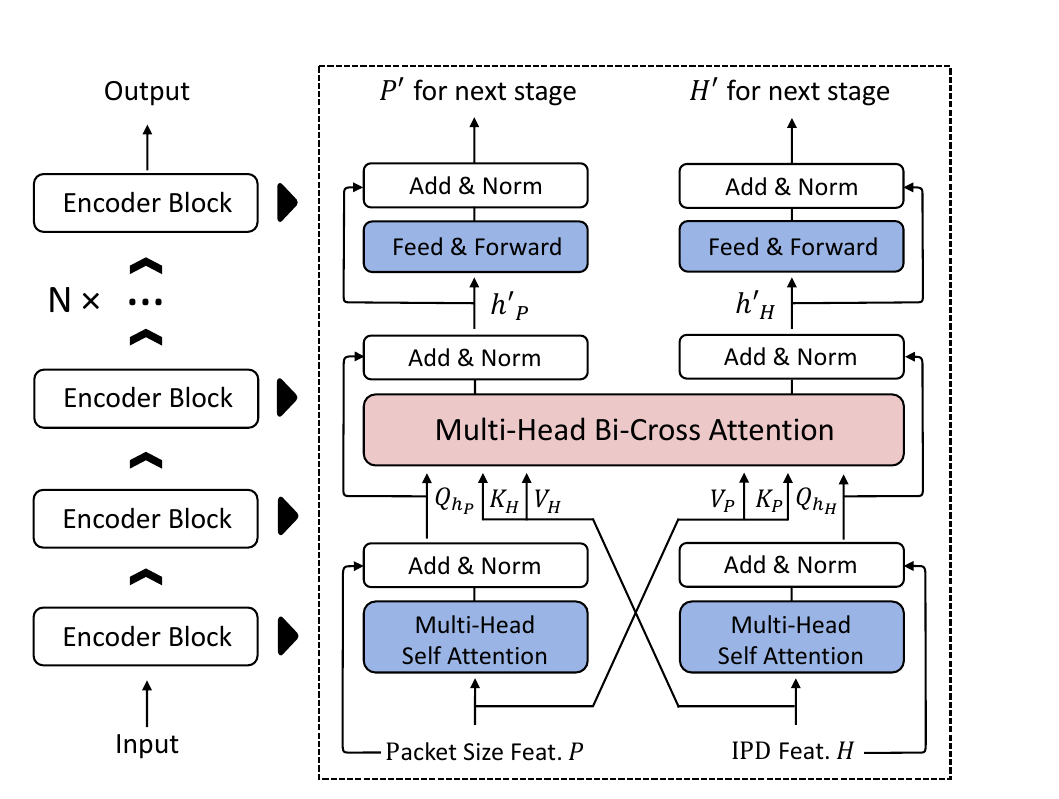
\includegraphics[width=\linewidth,height=5.9cm,keepaspectratio]{fig5.png}
\column{0.53\textwidth}
\begin{card}
  \cardtitle{Bi-Cross Attention}
  Каждый блок = self-attention (внутри последовательности) + двунаправленный cross-attention (размер $\leftrightarrow$ IPD) + FFN. Одна последовательность запрашивает другую и наоборот — та же сложность $O(n^2 d_k)$.
\end{card}\par\vspace{4mm}
\begin{darkcard}
  \iconitem{accent}{ic_flask_w.png}{\bfseries\small\color{accentlt}Задача Mask-Fill}\par\vspace{2mm}
  Маскируем 15\% позиций в обеих последовательностях сразу (80\% [MASK] / 10\% случайный / 10\% без изменений). Модель учится достраивать реалистичные benign-пакеты по контексту.
\end{darkcard}
\end{columns}
\end{frame}

% 13. MDP
\newcommand{\mdprow}[3]{%
  \begin{card}[top=1.5mm,bottom=1.5mm,left=2mm]
    \iconitem[0.55cm]{navy}{#1}{\hl{#2}\quad #3}
  \end{card}\par\vspace{1.9mm}}
\newcommand{\rewrow}[2]{{\headfont\bfseries\small\color{accentlt}#1}\par\vspace{0.6mm}
  {\scriptsize\color{cardline}#2}\par\vspace{0.8mm}{\color{steel}\rule{\linewidth}{0.4pt}}\par\vspace{2mm}}
\begin{frame}{Стадия 2 · Формализация как MDP}
\framesubtitle{Генерация adversarial-трафика = марковский процесс принятия решений}
\vspace{1mm}
\begin{columns}[T,onlytextwidth]
\column{0.62\textwidth}
  \mdprow{ic_layers_w.png}{Состояние $S$}{$(P_t, H_t)$ — текущие последовательности размеров и задержек}
  \mdprow{ic_random_w.png}{Действие $A$}{$2n{+}1$ вариантов: изменить пакет $i$ или вставить chaff-пакет}
  \mdprow{ic_gears_w.png}{Переход $P$}{детерминированный: Traffic-BERT заполняет [MASK]}
  \mdprow{ic_balance_w.png}{Награда $R$}{$r = r_E + \beta\, r_D + \gamma\, r_M$}
  \mdprow{ic_clock_w.png}{Горизонт $T$}{стоп при $t = \tau$ ($\le 10$) или достижении порога уклонения $\xi$}
\column{0.35\textwidth}
\begin{darkcard}[height=5.95cm]
  \cardtitlew{Награда: три части}\vspace{0.5mm}
  \rewrow{$r_E$}{доля пакетов, прошедших детектор (главная цель)}
  \rewrow{$\beta\, r_D$}{штраф непохожести: $-1$ за шаг $\rightarrow$ минимум правок}
  {\headfont\bfseries\small\color{accentlt}$\gamma\, r_M$}\par\vspace{0.6mm}
  {\scriptsize\color{cardline}штраф эффективности: сохраняет функцию атаки (напр. rate для DoS)}
\end{darkcard}
\end{columns}
\end{frame}

% 14. SAC
\newcommand{\step}[2]{%
  \par\noindent\tikz[baseline=(n.base)]\node[circle,fill=accent,text=white,inner sep=0pt,
    minimum size=0.42cm,font=\scriptsize\bfseries](n){#1};\hspace{2mm}#2\par\vspace{2.6mm}}
\begin{frame}{Стадия 2 · Оптимизация политики (SAC)}
\framesubtitle{Soft Actor-Critic: сильное исследование большого дискретного пространства}
\vspace{1mm}
\begin{columns}[T,onlytextwidth]
\column{0.56\textwidth}
\begin{card}[height=5.9cm]\scriptsize
  \cardtitle{Почему такой выбор}
  \iconitem[0.55cm]{steel}{ic_gears_w.png}{\hl{GRU-политика}\ \ лёгкая RNN: понимает последовательность, быстро обучается}\vspace{3.2mm}
  \iconitem[0.55cm]{steel}{ic_balance_w.png}{\hl{Двойные Q-сети}\ \ снижают переоценку значений действий}\vspace{3.2mm}
  \iconitem[0.55cm]{steel}{ic_random_w.png}{\hl{Invalid Action Masking}\ \ отсекает недопустимые позиции ($n >$ длины потока)}\vspace{3.2mm}
  \iconitem[0.55cm]{steel}{ic_brain_w.png}{\hl{Traffic-BERT «заморожен»}\ \ часть среды $\rightarrow$ обучение развязано и дешевле}
\end{card}
\column{0.41\textwidth}
\begin{wcard}[height=5.9cm]\scriptsize
  \cardtitle{Один шаг обучения}\vspace{0.5mm}
  \step{1}{Политика выбирает действие $a_t$}
  \step{2}{Вставка / замена на [MASK]}
  \step{3}{Traffic-BERT заполняет $\rightarrow s_{t+1}$}
  \step{4}{Отправка потока, замер награды}
  \step{5}{Транзиция в replay-буфер}
  \step{6}{Обновление Q-сетей и политики}
\end{wcard}
\end{columns}
\end{frame}

% 15. Без обратной связи
\begin{frame}{Стадия 2 · Атака без обратной связи}
\framesubtitle{На инференсе метки может не быть — оцениваем награду офлайн}
\vspace{2mm}
\begin{card}[top=3mm,bottom=3mm]
  \iconitem{steel}{ic_eye_w.png}{\hl{Проблема:} во время реальной атаки детектор не всегда даёт сигнал «прошёл / не прошёл» — нельзя понять, когда останавливаться.}
\end{card}\par\vspace{4mm}
\begin{darkcard}[top=3mm,bottom=3mm]
  \iconitem{accent}{ic_check_w.png}{{\bfseries\color{accentlt}Решение:} аппроксимируем ожидаемую награду максимумом из двух обученных Q-сетей и останавливаемся по порогу $\xi'$ (взят из фазы обучения).}
\end{darkcard}\par\vspace{4mm}
\begin{card}[colback=cardline!60,colframe=cardline!60,halign=flush center,top=4mm,bottom=4mm]
  {\headfont\bfseries\normalsize\color{navy}Условие остановки: \quad
   $(t \ge \tau) \;\lor\; \bigl(\max_i Q_{\omega_i}(s_t, a_t) \ge \xi'\bigr)$}
\end{card}
\end{frame}

% 16. Постановка экспериментов
\newcommand{\statbox}[5]{% bg, number color, number, label, sublabel
  \begin{tcolorbox}[nmbase,colback=#1,colframe=#1,halign=flush center,height=1.95cm,valign=center]
    {\headfont\bfseries\fontsize{19}{21}\selectfont\color{#2}#3}\par\vspace{1mm}
    {\scriptsize\bfseries\ifstrequal{#1}{navy}{\color{white}}{\color{navy}} #4}\par\vspace{0.3mm}
    {\tiny\ifstrequal{#1}{navy}{\color{cardline}}{\color{muted}} #5}
  \end{tcolorbox}}
\begin{frame}{Постановка экспериментов}
\vspace{1mm}
\begin{columns}[T,onlytextwidth]
\column{0.235\textwidth}\statbox{navy}{accentlt}{6}{детекторов-целей}{3 традиционных ML + 3 DL}
\column{0.235\textwidth}\statbox{cardbg}{accent}{80}{сценариев атак}{12 типов трафика × методы}
\column{0.235\textwidth}\statbox{navy}{accentlt}{12}{типов трафика}{скан, DoS, ботнеты, веб-атаки}
\column{0.235\textwidth}\statbox{cardbg}{accent}{4}{базовых метода}{R.M., M.I., \mbox{Traffic Manipulator}, Amoeba}
\end{columns}
\vspace{3.5mm}
\begin{columns}[T,onlytextwidth]
\column{0.485\textwidth}
\begin{wcard}[height=3.3cm]\scriptsize
  \cardtitle{Данные и стенд}
  \iconitem[0.5cm]{steel}{ic_network_w.png}{Фон — WIDE MAWI (июнь/август 2023), >1 млн потоков}\vspace{2mm}
  \iconitem[0.5cm]{steel}{ic_server_w.png}{PyTorch + Intel DPDK, Xeon Gold 6348, A100, NIC 2×10 Гбит/с}\vspace{2mm}
  \iconitem[0.5cm]{steel}{ic_book_w.png}{Датасеты: Kitsune, PeerRush, HyperVision (только публичные)}
\end{wcard}
\column{0.485\textwidth}
\begin{wcard}[height=3.3cm]\scriptsize
  \cardtitle{Метрики}
  \iconitem[0.5cm]{accent}{ic_bullseye_w.png}{\hl{ASR} — доля вредоносных потоков, не пойманных детектором}\vspace{2mm}
  \iconitem[0.5cm]{accent}{ic_chart_w.png}{\hl{AUC / F1} — качество самих детекторов без атаки}\vspace{2mm}
  \iconitem[0.5cm]{accent}{ic_tacho_w.png}{\hl{Bandwidth} (Mbps) и \hl{throughput} (PPS) — влияние и скорость}
\end{wcard}
\end{columns}
\end{frame}

% 17. Главный результат
\begin{frame}{Главный результат: успех атаки (ASR)}
\framesubtitle{В 56 из 72 сценариев — лучший результат среди всех методов}
\vspace{1mm}
\begin{columns}[T,onlytextwidth]
\column{0.3\textwidth}
\begin{darkcard}[height=5.9cm,halign=flush center]
  \vspace{4mm}
  {\scriptsize\color{white}в среднем}\par\vspace{3mm}
  {\headfont\bfseries\fontsize{24}{26}\selectfont\color{accentlt}96.65\%}\par\vspace{3mm}
  {\scriptsize\color{white}успешных уклонений}\par\vspace{3mm}
  {\color{steel}\rule{0.85\linewidth}{0.5pt}}\par\vspace{7mm}
  {\scriptsize\color{white}ASR по детекторам: 0.96–0.99\\против 6 систем}
\end{darkcard}
\column{0.66\textwidth}
  {\small\bfseries\color{navy}Прирост ASR над лучшим базовым методом, \%}\par\vspace{3mm}
  \begin{tikzpicture}[x=0.285cm,y=0.72cm,font=\scriptsize]
    \foreach \name/\val/\c [count=\i] in {
        Whisper/2.61/steel, FlowLens/3.11/steel, NetBeacon/15.53/accent,
        Vanilla+RNN/21.88/accent, CICFlowMeter/20.78/accent, Kitsune/14.42/accent} {
      \pgfmathsetmacro{\yy}{-\i}
      \node[anchor=east,text=ink] at (-0.4,\yy) {\name};
      \fill[\c,rounded corners=0.6pt] (0,\yy-0.24) rectangle (\val,\yy+0.24);
      \node[anchor=west,text=ink,font=\scriptsize\bfseries] at (\val+0.25,\yy) {+\val};
    }
  \end{tikzpicture}\par\vspace{2mm}
  \figcap{Наибольший выигрыш — против DL-детекторов, где базовые атаки слабы.}
\end{columns}
\end{frame}


\end{document}